\documentclass[12pt]{article}
\usepackage{hyperref} 
\usepackage{titling}
\usepackage{xcolor}
\usepackage[a4paper,margin=1in]{geometry}
\usepackage{fancyhdr}
\usepackage{graphicx}
\usepackage{tabto}
\pagestyle{fancy}
\chead{Final Report}
\lhead{}
\rhead{}
\graphicspath{ {./images/} }
\usepackage{pdfpages}

\begin{document}
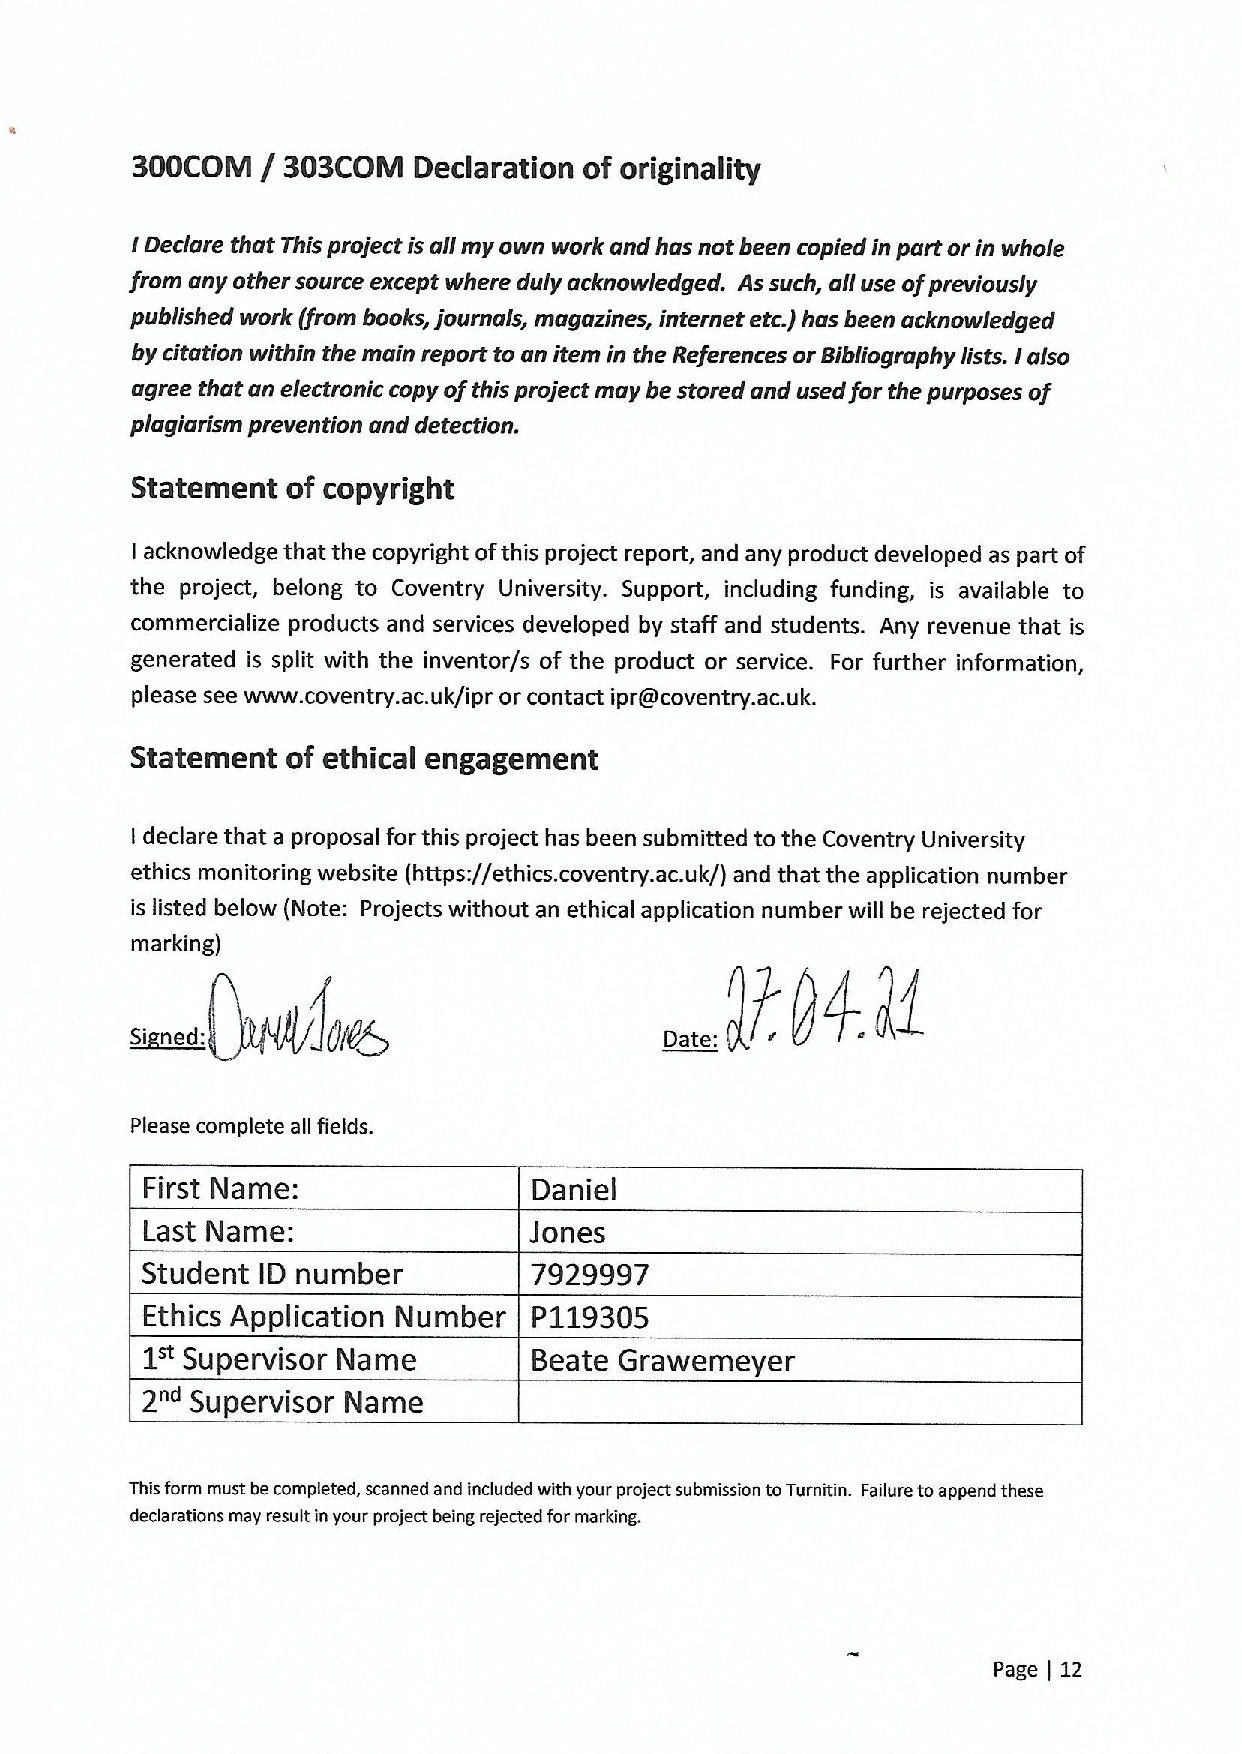
\includepdf[pages=-]{SER_Daniel_Jones_Declaration.pdf}
\begin{center}
	\vspace*{1cm}
	\Huge \textbf{A Speech Emotion Recognition Classifier to Aid Performance Review in Learning Environments} \\[1em]
	\vspace{5cm}
	\LARGE \textbf{Daniel G. Jones}
	\\
	\vspace{0.3cm}
	\large jonesd37@coventry.ac.uk
	\\
	\large Student ID: 7929997
	\\
	\vspace{3cm}
	\large Supervised by \textbf{Dr. Beate Grawemeyer}
	\\
	\vspace{0.3cm}
	\large ac7655@coventry.ac.uk
	\\
	\vspace{3cm}
	\large Submitted to the School of Computing, Engineering and Mathematics Coventry University
\end{center}
\newpage
\tableofcontents
\newpage
\section{Abstract}

Classifying human emotion from speech is a challenging problem that has the potential to benefit various fields in different ways. One such field is in learning environments, where the application of such technology could aid in matters such as performance review / analysis or in helping children with special needs, such as autism. In this project, a speech emotion classification model has been built, trained, and deployed in the form of a graphical tool that analyses either pre-recorded audio or a live audio input and outputs the weighted predictions. The model has been developed using a 2-Dimensional Convolutional Neural Network (CNN) approach, where the training data is in the form of audio files converted into Mel Spectrograms. Through this approach, an exact prediction accuracy of 68.8\% (and binary positive / negative accuracy of 94\%) has been achieved on an unseen test dataset, with further personalised tests yielding promising results.

\section{Acknowledgements}

With thanks to my project supervisor, Dr. Beate Grawemeyer, for the initial inspiration and constant support throughout the project.
\\

\noindent With thanks to my friend Céline Capelli of ETH Zürich for testing the application, providing useful audio data for testing, and for offering her unique perspective.
\\

\noindent With thanks to my partner Hannah Vogt of the Pädagogische Hochschule Zürich for her love, inspiration, motivation, and for offering the insights of a primary school teacher. 
\\
\newpage

\section{Introduction}

It can be observed that technology has yet to make a significant contribution towards aiding performance review in learning environments and indeed learning environments on the whole. This can largely be attributed to the lack of effectiveness of the existing tools, whereby much of the information obtained is neither insightful nor particularly meaningful.
\\

\noindent Traditional approaches to the incorporation of technology in learning environments have tended to focus more on interactivity as opposed to analysis, which has resulted in a lack of progress in the areas of performance review, analysis, and overall utility. This is due to the complexity of such environments, with many subjective metrics and mediums that, at first glance, appear to be difficult to study and quantify.
\\

\noindent In this project, speech emotion has been identified and selected as a suitable metric for analysis. Speech emotion is a language agnostic metric that transcends many of the barriers posed by the more obvious metrics such as spoken / body language or facial expressions.
\\

\noindent Despite the many nuances of speech, such as tonality or pitch, there are clear patterns that can be detected when studying how emotions are conveyed. A spectrogram is a visual representation of the spectrum of frequencies across a signal as a function of time. Consider the following two spectrograms of two different men saying a short sentence in a blatantly angry manner. 
\\

\newpage

\noindent \textbf{Gantt Chart}
\\
\noindent In order to illustrate the schedule of the project, I have produced a Gantt chart, shown below.
\\
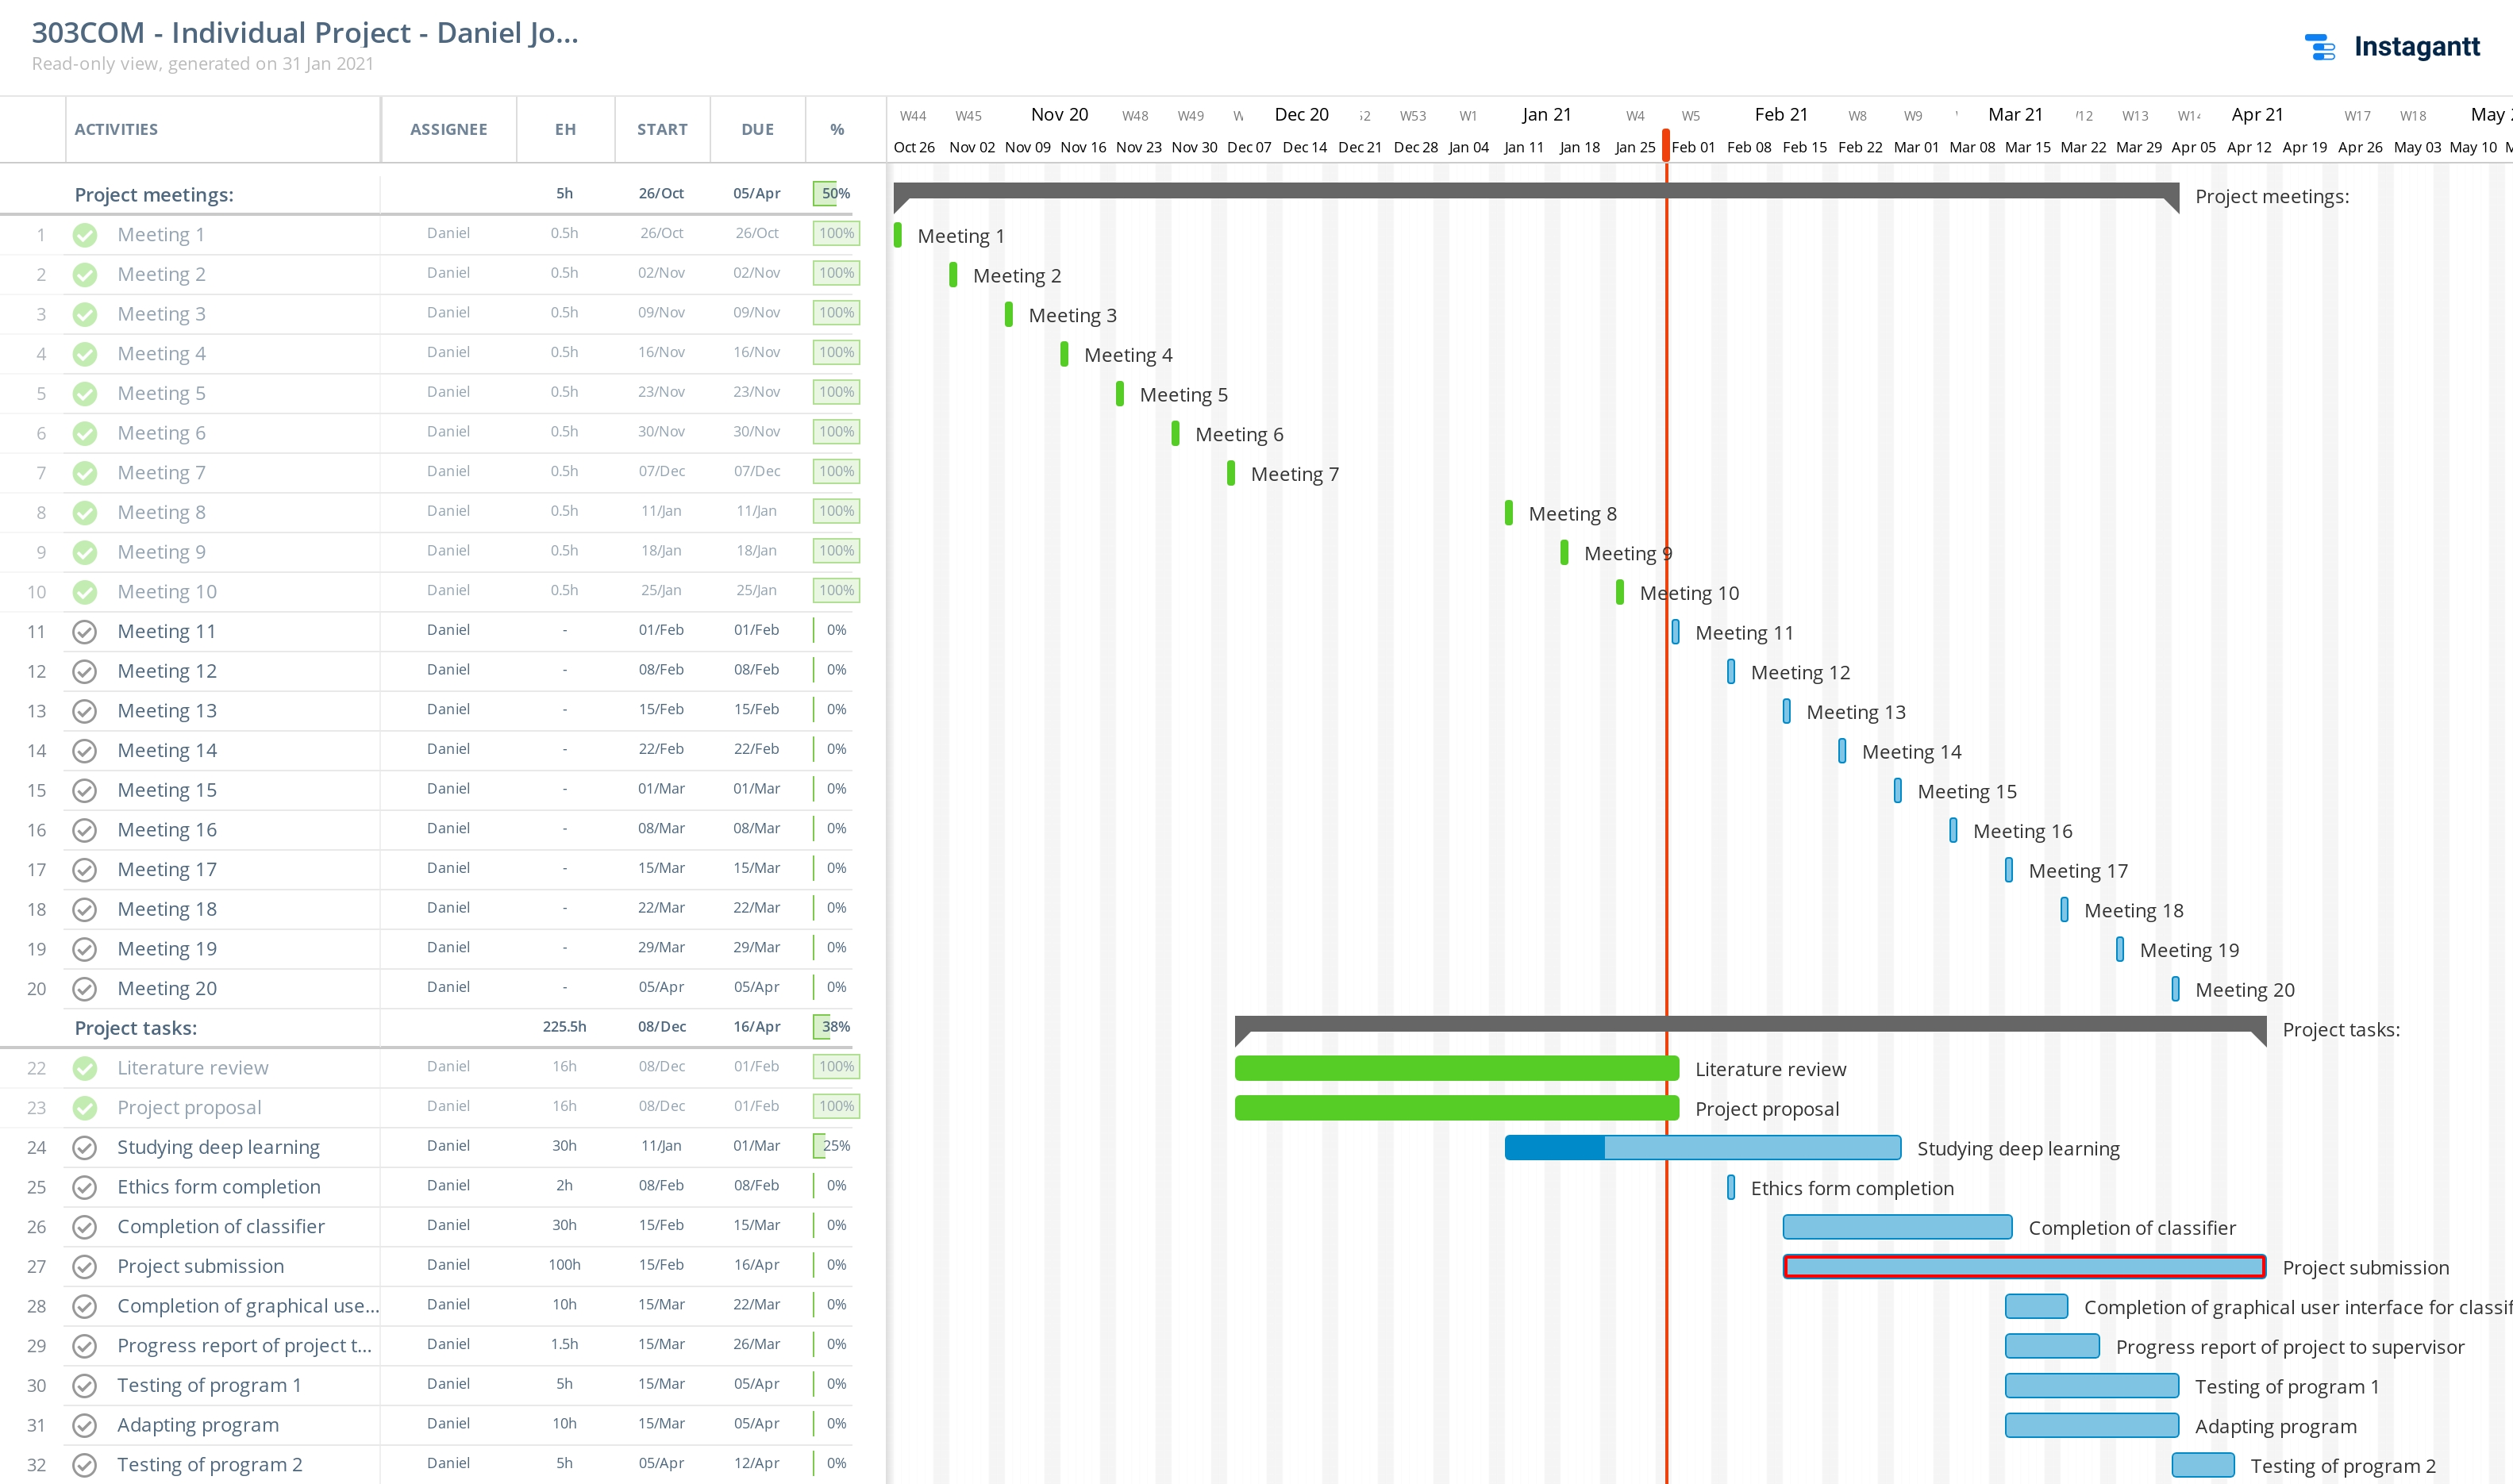
\includegraphics[width=18cm, height=12cm]{Daniel_Jones_Gantt_Chart}
\\
\noindent \href{https://i.imgur.com/9tchO4N.jpg}{\color{blue}\textbf{Link to full size image}}
\\
\noindent \href{https://app.instagantt.com/shared/s/PdaKZZeApqszVu1eftjC/latest}{\color{blue}\textbf{Link to latest edition of the chart}}
\\
\pagebreak

\noindent \textbf{5. Initial Literature Review}
\\
The first set of literature has been selected with development, methodologies, and comparisons between Speech Emotion Recognition (SER) technologies in mind. From the perspective of a beginner, starting with such papers makes sense; it enables one to develop an initial understanding of the current methods and strategies used to tackle the problem of SER.
\\

\noindent \href{https://www.intechopen.com/books/social-media-and-machine-learning/automatic-speech-emotion-recognition-using-machine-learning}{\textbf{Automatic Speech Emotion Recognition Using Machine Learning}}
\\
The first paper, Automatic Speech Emotion Recognition Using Machine Learning (2019), takes a comparative look at SER systems. The underlying method to extract and process the speech signals (using Mel-frequency cepstrum coefficients and modulation spectral features in conjunction with feature selection) remains the same whilst the machine learning paradigms differ. The paper first looks at a recurrent neural network approach and goes on to compare it against both multivariate linear regression and support vector machine approaches. The paper makes the claim that such approaches were selected due to their existing popularity in the field. 
\\

\noindent The initial criticism of the paper is that it fails to consider the convolutional neural network (CNN) approach, despite its notable popularity and differences to the other methods. However, the paper is still concise and informative enough to warrant a full review. One positive quality that immediately stands out is how clear the information is presented, both in terms of looks and in use of language. An additional outstanding quality of this paper is the lack of pre-requisite knowledge required of the reader; many similar such papers assume at least a fundamental understanding and generally a lot more, whilst this paper describes most of the necessary knowledge required to grasp the content.
\\

\noindent The paper starts by explaining the importance behind SER technology, the main argument can be reduced to how effective and convenient it is to obtain information pertaining to the emotional state of an individual in comparison to other methods (such as facial expressions and physiological signals). This argument can be applied to the idea of using such technology in learning environments based on the documented effectiveness of the results in similar scenarios. The paper even uses learning environments as an example of a potential application of such technology: ``a teacher can use SER to decide what subjects can be taught and must be able to develop strategies for managing emotions within the learning environment.'' (Kerkeni et al., 2019, p. 2).
\\

\noindent The authors then describe their system from a top-down perspective, this includes which emotions are in scope as well as the decision making process behind which algorithms are selected. It appears that the researchers were restricted by their datasets as to which emotions ended up in-scope. Whilst this does not affect the content of this particular paper, a more careful consideration will have to be made when applying this to learning environments (as per this project).
\\

\noindent Delving further into the paper, the authors describe how the different algorithms are applied to solve the problem, which is achieved by mathematical notation and descriptions of important variables. This is of course a necessity for such a paper, although the notation is clear enough for even those with weaker mathematical backgrounds to gain insight. The paper concludes by displaying and contrasting between the results obtained from the experiments; the main conclusion is that SER produces the best recognition results with a limited dataset whilst RNN performs better when a higher volume of data is available. Such results will prove vital when comparing against and assessing the effectiveness of our SER system.
\\

\noindent \href{https://www.mdpi.com/1424-8220/20/1/183/pdf}{\textbf{A CNN-Assisted Enhanced Audio Signal Processing for Speech Emotion Recognition}}
\\
Due to the notable omission of a CNN approach in the first reviewed paper, this paper has primarily been selected to gain practical insight into such an approach. The paper starts by defining the motivation behind it, using similar arguments to the previously reviewed paper. One particular area of interest is the point about ``extracting hidden information'' (Kwon, S. 2020, p. 1), where the author refers to uncovering previously undetected, new information using a CNN approach. At first glance, it appears that the author looks at the issue more through the lens of human computer interaction (HCI), contrasting with the previous paper's theoretical approach.
\\

\noindent An immediate positive point of the paper is that it describes its approach clearly and in plenty of detail, though unlike the first paper, this paper requires the reader to possess fundamental knowledge concerning machine learning terminology and methods. The paper goes on to discuss the proposed methodology, which is essentially a model comprising of input layers (taking in 2D speech signal spectrograms), several convolutional layers flattened down, and two fully connected layers with the softmax classifier applied at the end. Compared to the first paper, this approach seems easier and requires a lot less pre-processing work applied to a given dataset (since the audio just needs transforming into a 2d spectrograph). The main downside to this paper is that it lacks technical and theoretical insight, providing only a single equation unrelated to the classifier itself.
\\

\noindent Cutting to the end results of the paper, given the clear lack of training applied to the model, the results achieved are not bad. Although lower than one might expect given some of the cutting-edge results achieved through CNNs on other projects; the lack of training surely impacts this. In conclusion, the paper has provided an insightful and inspiring approach to be considered for this project. As with the prior paper, the end results will be interesting to compare against in the end. 
\\
\pagebreak
\\

\noindent This next section of literature focuses more on the learning environment side of the project. The purpose of this is to justify the motivations behind the project and to refine and further develop the research questions.
\\

\noindent \href{https://files.eric.ed.gov/fulltext/EJ1194723.pdf}{\textbf{Factors Affecting Technology Integration in the Classroom}}
\\
This paper provides solid reasoning on the critical factors affecting the integration of technology in learning environments. The paper consists of 5 key reasons as to why classrooms benefit less from technology than many other environments: poor infrastructure, inadequate technology, lack of sufficient, effective professional development, low self-efficacy, and teacher perceptions. Each reason stated in the paper is insightful, but the points regarding inadequate technology and teacher perceptions are of the most relevance to the project. As previously mentioned, one of the goals of this project would be to put forth a valid and viable application of technology in learning environments (as to build some interest around the idea). The paper states that teachers ``perceive the effort needed to learn the new technology and practicality of it as a significant consideration in whether they use it or not'' (Harrell, S., \& Bynum, Y. 2018. p. 15), so in order for this to work, the educators must be convinced of the technology.
\\

\noindent \href{https://www.researchgate.net/profile/Ryan-Baker-2/publication/326217846_Modeling_Learners'_Cognitive_and_Affective_States_to_Scaffold_SRL_in_Open-Ended_Learning_Environments/links/5b560a4245851507a7c3f516/Modeling-Learners-Cognitive-and-Affective-States-to-Scaffold-SRL-in-Open-Ended-Learning-Environments.pdf}{\textbf{Modeling learners' cognitive and affective states to scaffold SRL in open-ended learning environments}}
\\
Whilst this paper largely covers an area unrelated to the project, the points regarding relationships between cognitive and affective states are interesting and will be of use to the analysis stage of the project. The paper goes on to describe an interesting correlation between two affective states, boredom and delight, and academic performance. As one might expect, an exposed state of boredom significantly decreases cognitive and subsequently academic performance, as documented by the paper. With these statistics in mind, prioritising the prediction of the states of boredom and delight from speech will be areas of particular interest to focus training the model on.

\pagebreak
\noindent \textbf{6. Bibliography}
\\
\noindent Harrell, S., \& Bynum, Y. (2018). Factors affecting technology integration in the \tab \tab classroom. \textit{Alabama Journal of Educational Leadership}, 5, 12-18
\\

\noindent Kerkeni, L., Serrestou, Y., Mbarki, M., Raoof, K., Mahjoub, M.A. \& Cleder, C. (2019). \tab \tab Automatic Speech Emotion Recognition Using Machine Learning. In \textit{Social media \tab \tab and machine learning}. IntechOpen. \href{https://doi.org/10.5772/intechopen.84856}{https://doi.org/10.5772/intechopen.84856}.
\\

\noindent Kwon, S. (2020). A CNN-assisted enhanced audio signal processing for speech emotion \tab \tab recognition. \textit{Sensors}, 20(1), 183. \href{http://doi.org/10.3390/s20010183}{http://doi.org/10.3390/s20010183}.
\\

\noindent Munshi, A., Rajendran, R., Ocumpaugh, J., Biswas, G., Baker, R. S., \& Paquette, L. \tab \tab (2018, July). Modeling learners' cognitive and affective states to scaffold SRL in open-\tab \tab ended learning environments. In \textit{Proceedings of the 26th conference on user modeling, \tab \tab adaptation and personalization} (pp. 131-138). \href{https://doi.org/10.1145/3209219.3209241}{https://doi.org/10.1145/3209219.3209241}

\end{document}